\documentclass[aspectratio=169,xcolor=table]{beamer}
\usepackage[utf8]{inputenc}
\usepackage[T1,T5]{fontenc}
\usepackage{amsmath,booktabs,array,graphicx,pifont}

\definecolor{Primary}{HTML}{111B88}
\definecolor{Secondary}{HTML}{101659}
\definecolor{Accent}{HTML}{F2A900}
\definecolor{SoftBlue}{HTML}{EAF2F8}
\definecolor{TextGray}{HTML}{4D5966}
\definecolor{RiskRed}{HTML}{A23B3B}
\definecolor{GoodGreen}{HTML}{26734D}
\mode<presentation>{\usetheme{Madrid}\usecolortheme{default}\setbeamertemplate{navigation symbols}{}}
\setbeamercolor{structure}{fg=Primary}
\setbeamercolor{frametitle}{fg=white,bg=Primary}
\setbeamercolor{title}{fg=white,bg=Primary}
\setbeamercolor{block body}{fg=black,bg=SoftBlue}
\setbeamercolor{block body alerted}{fg=black,bg=Accent!12}
\setbeamercolor{section in head/foot}{fg=white,bg=Primary}
\setbeamercolor{author in head/foot}{fg=white,bg=Secondary}
\setbeamercolor{date in head/foot}{fg=white,bg=Primary}
\setbeamerfont{section in head/foot}{size=\tiny,series=\bfseries}
\setbeamerfont{author in head/foot}{size=\scriptsize}
\setbeamerfont{date in head/foot}{size=\scriptsize,series=\bfseries}
\setbeamerfont{frametitle}{series=\bfseries}
\setbeamerfont{title}{series=\bfseries}
\newcommand{\decklabel}{Scorer bias word 17/10/2026}
\setbeamertemplate{itemize item}{\color{Secondary}$\blacktriangleright$}
\setbeamertemplate{itemize subitem}{\color{Accent}$\bullet$}
\setbeamertemplate{headline}{\leavevmode\begin{beamercolorbox}[wd=\paperwidth,ht=2.7ex,dp=1.1ex,leftskip=.35cm,rightskip=.35cm]{section in head/foot}\insertsectionnavigationhorizontal{\dimexpr\paperwidth-.70cm\relax}{}{}\end{beamercolorbox}}
\setbeamertemplate{footline}{\leavevmode\hbox{\begin{beamercolorbox}[wd=.55\paperwidth,ht=2.6ex,dp=1ex,leftskip=.35cm,rightskip=.20cm]{section in head/foot}\usebeamerfont{section in head/foot}\insertsectionhead\end{beamercolorbox}\begin{beamercolorbox}[wd=.27\paperwidth,ht=2.6ex,dp=1ex,center]{author in head/foot}\usebeamerfont{author in head/foot}\decklabel\end{beamercolorbox}\begin{beamercolorbox}[wd=.18\paperwidth,ht=2.6ex,dp=1ex,rightskip=.35cm plus1fil]{date in head/foot}\usebeamerfont{date in head/foot}\hfill\insertframenumber\,/\,\inserttotalframenumber\end{beamercolorbox}}}
\newcommand{\hi}[1]{\textcolor{Primary}{\textbf{#1}}}
\newcommand{\bad}[1]{\textcolor{RiskRed}{\textbf{#1}}}
\newcommand{\good}[1]{\textcolor{GoodGreen}{\textbf{#1}}}
\newcommand{\src}[1]{{\tiny\color{TextGray}[#1]}}

\title{Scorer chấm bias word theo audio}
\subtitle{Audio + bias list $\rightarrow$ xác suất mỗi từ có trong audio}
\author{Nhóm Contextual ASR}
\institute{}
\date{17/10/2026}
\setbeamertemplate{title page}{\begin{centering}\vspace*{0.10cm}
\includegraphics[height=1.08cm]{imgs/logo.png}\par\vspace{0.32cm}\begin{beamercolorbox}[sep=0.50em,center,rounded=true]{title}\usebeamerfont{title}\inserttitle\par\vspace{0.14cm}{\small\insertsubtitle\par}\end{beamercolorbox}\vspace{0.42cm}{\usebeamerfont{author}\insertauthor\par}\vspace{0.10cm}{\usebeamerfont{institute}\insertinstitute\par}\vfill{\usebeamerfont{date}\insertdate\par}\end{centering}}

\begin{document}
\begin{frame}[plain]\titlepage\end{frame}

\section{Việc được giao}
\begin{frame}{Mục tiêu và tiến độ}
\begin{beamercolorbox}[sep=0.6em,rounded=true]{block body}
\textbf{Mục tiêu:} một \hi{scorer} nhận \textbf{audio} và \textbf{bias list}, chấm cho mỗi từ khả năng từ đó xuất hiện trong audio.
\end{beamercolorbox}
\vspace{0.35cm}
\begin{itemize}\itemsep6pt
\item \good{Đã làm xong và train xong} trên LibriSpeech train-clean-100 (28.539 câu).
\item Đầu ra là \textbf{xác suất} $\in[0,1]$ = sigmoid(điểm khớp giữa âm vị của từ và audio); học bằng nhãn có / không của dữ liệu train.
\item Đo 2 tầng trên benchmark IS21 (giống Hou25 / PTC-Bias):
  \begin{itemize}
  \item \textbf{Scorer tự thân:} chọn đúng bao nhiêu từ?
  \item \textbf{Đưa vào Qwen3-ASR:} B-WER giảm bao nhiêu?
  \end{itemize}
\end{itemize}
\vspace{0.2cm}
\begin{beamercolorbox}[sep=0.5em,rounded=true]{block body alerted}
\small\textbf{Kết quả chính:} list 2000 từ $\rightarrow$ còn $\sim$3 từ/câu, giữ \textbf{95\%} từ đúng; B-WER của Qwen \textbf{7,40 $\rightarrow$ 4,78} (oracle 4,01).
\end{beamercolorbox}
\end{frame}

\section{Bài toán}
\begin{frame}{Bài toán: vì sao có bias list dài, và vì sao cần chọn lọc}
\begin{columns}[T]
\begin{column}{0.52\textwidth}
\small
\textbf{ASR sai ở từ hiếm} (tên riêng, thuật ngữ):\\[2pt]
\quad nói: \emph{``missus \textbf{neverbend} you must\dots''}\\
\quad Qwen: \emph{``missus \bad{never been} you must\dots''}\\[6pt]
\textbf{Cách chữa:} nhắc trước một \hi{bias list} các từ có thể xuất hiện.\\[6pt]
\textbf{Ngoài đời list dài vì không biết trước người dùng sẽ nói gì:}
\begin{itemize}\itemsep1pt
\item gọi điện: cả \textbf{danh bạ} (vài trăm--vài nghìn tên)
\item họp: tên mọi người + dự án trong công ty
\end{itemize}
$\Rightarrow$ mỗi câu chỉ 1--2 từ đúng, còn lại là \textbf{từ nhiễu}.
\end{column}
\begin{column}{0.46\textwidth}
\small
\textbf{Benchmark IS21} (Le et al.\ 2021) trên LibriSpeech:
\begin{itemize}\itemsep1pt
\item từ hiếm = ngoài 5.000 từ thông dụng
\item list mỗi câu = \good{từ hiếm thật của câu} + \bad{N từ hiếm ngẫu nhiên} (kho 209k), N = 100 \dots\ 2000
\end{itemize}
\vspace{2pt}
\renewcommand{\arraystretch}{1.15}
\begin{tabular}{@{}lc@{}}
\toprule
Qwen3-ASR, test-clean & B-WER\\
\midrule
không list & 7,40\\
\good{chỉ từ đúng} (oracle) & \good{4,01}\\
list N = 100 & 5,30\\
list N = 2000 & \bad{7,40}\\
\bottomrule
\end{tabular}\\[3pt]
\footnotesize B-WER = \% từ hiếm bị chép sai. List càng dài, Qwen càng rối $\rightarrow$ \hi{cần scorer chọn lọc}.
\end{column}
\end{columns}
\end{frame}

\section{Kiến trúc}
\begin{frame}{Kiến trúc scorer}
\centering
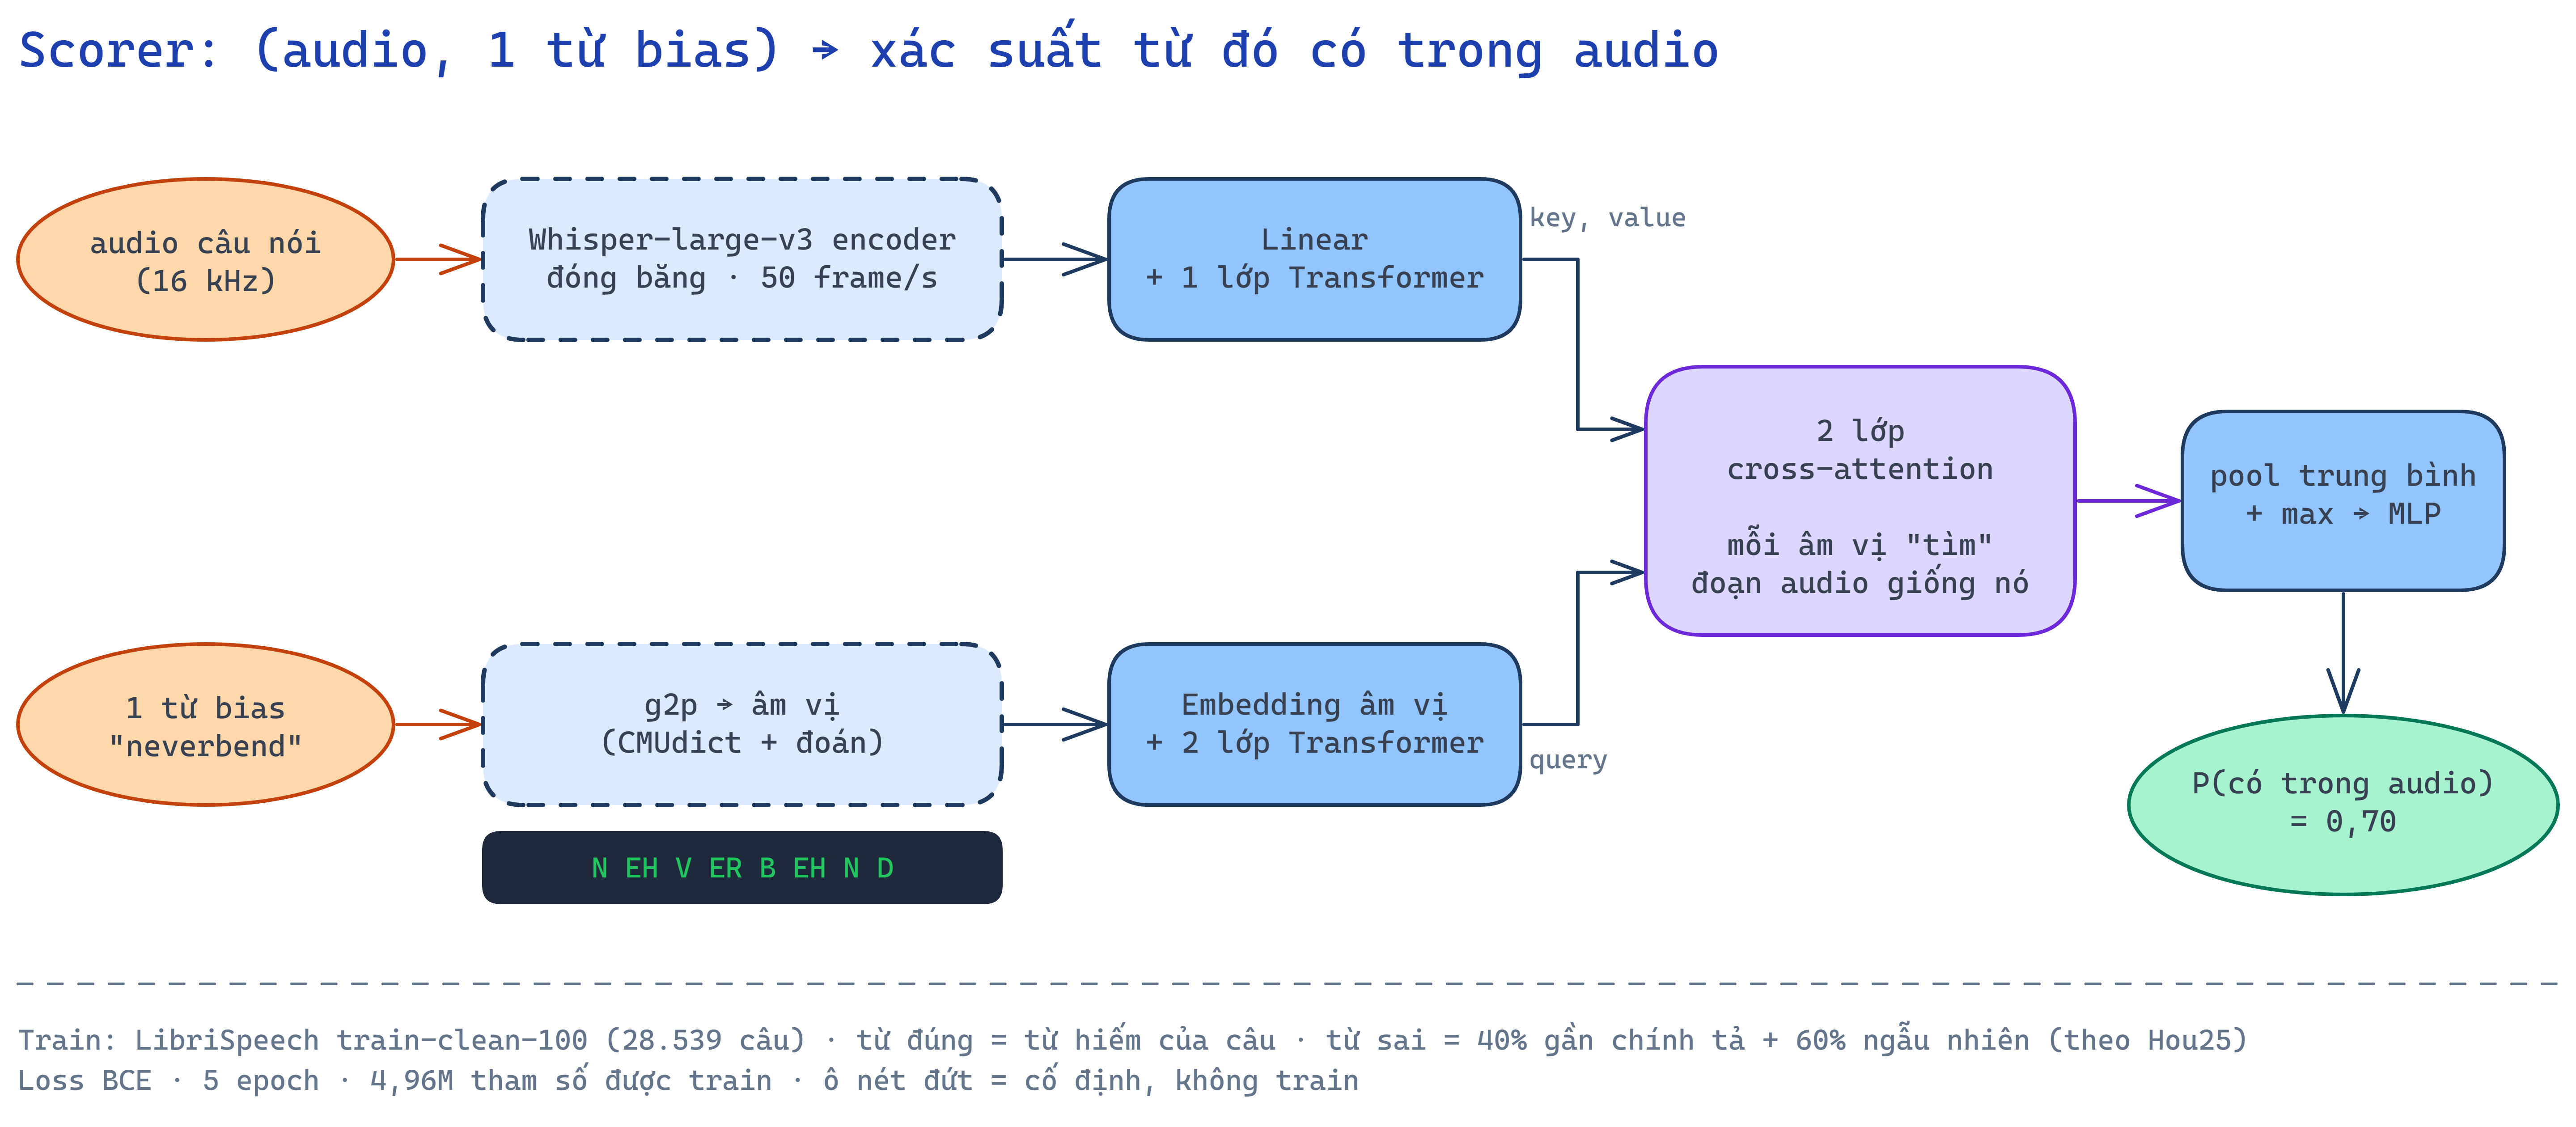
\includegraphics[height=0.72\textheight]{imgs/scorer_arch.png}\\[2pt]
{\footnotesize Khác Hou25: từ biểu diễn bằng \hi{âm vị} thay vì audio TTS $\rightarrow$ từ bất kỳ (kể cả LLM sinh) chấm được ngay; đầu ra là \hi{xác suất} $\rightarrow$ lọc theo ngưỡng được.}
\end{frame}

\begin{frame}{Từng khối làm gì}
\footnotesize\renewcommand{\arraystretch}{1.2}
\begin{tabular}{@{}>{\raggedright}p{3.6cm}p{9.4cm}c@{}}
\toprule
\textbf{Khối} & \textbf{Làm gì / vì sao} & \textbf{Train?}\\
\midrule
Whisper-large-v3 encoder & audio $\rightarrow$ 50 vector/giây (1280 chiều), mỗi vector mô tả âm thanh của 20 ms. Dùng sẵn, đủ tốt. & không\\
Linear + 1 lớp Transformer & đưa vector audio về 256 chiều, dạng scorer dễ so & có\\
g2p & từ $\rightarrow$ chuỗi âm vị: neverbend $\rightarrow$ N EH V ER B EH N D. Tra CMUdict, từ lạ thì đoán & không\\
Embedding âm vị + 2 lớp Transformer & mỗi âm vị $\rightarrow$ vector 256 chiều, biết ngữ cảnh âm vị bên cạnh & có\\
\hi{2 lớp cross-attention} & mỗi âm vị ``hỏi'' tất cả frame audio: \emph{đoạn nào giống tôi?} Nếu từ được nói, các âm vị tìm thấy đoạn khớp & có\\
Pool trung bình + max $\rightarrow$ MLP & gộp kết quả của các âm vị $\rightarrow$ 1 điểm $\rightarrow$ sigmoid $\rightarrow$ xác suất & có\\
\bottomrule
\end{tabular}\\[4pt]
\footnotesize Tổng 4,96M tham số được train. Code: \texttt{scorer/models.py} (\texttt{PhoneXAttn}).
\end{frame}

\begin{frame}{Train thế nào}
\centering
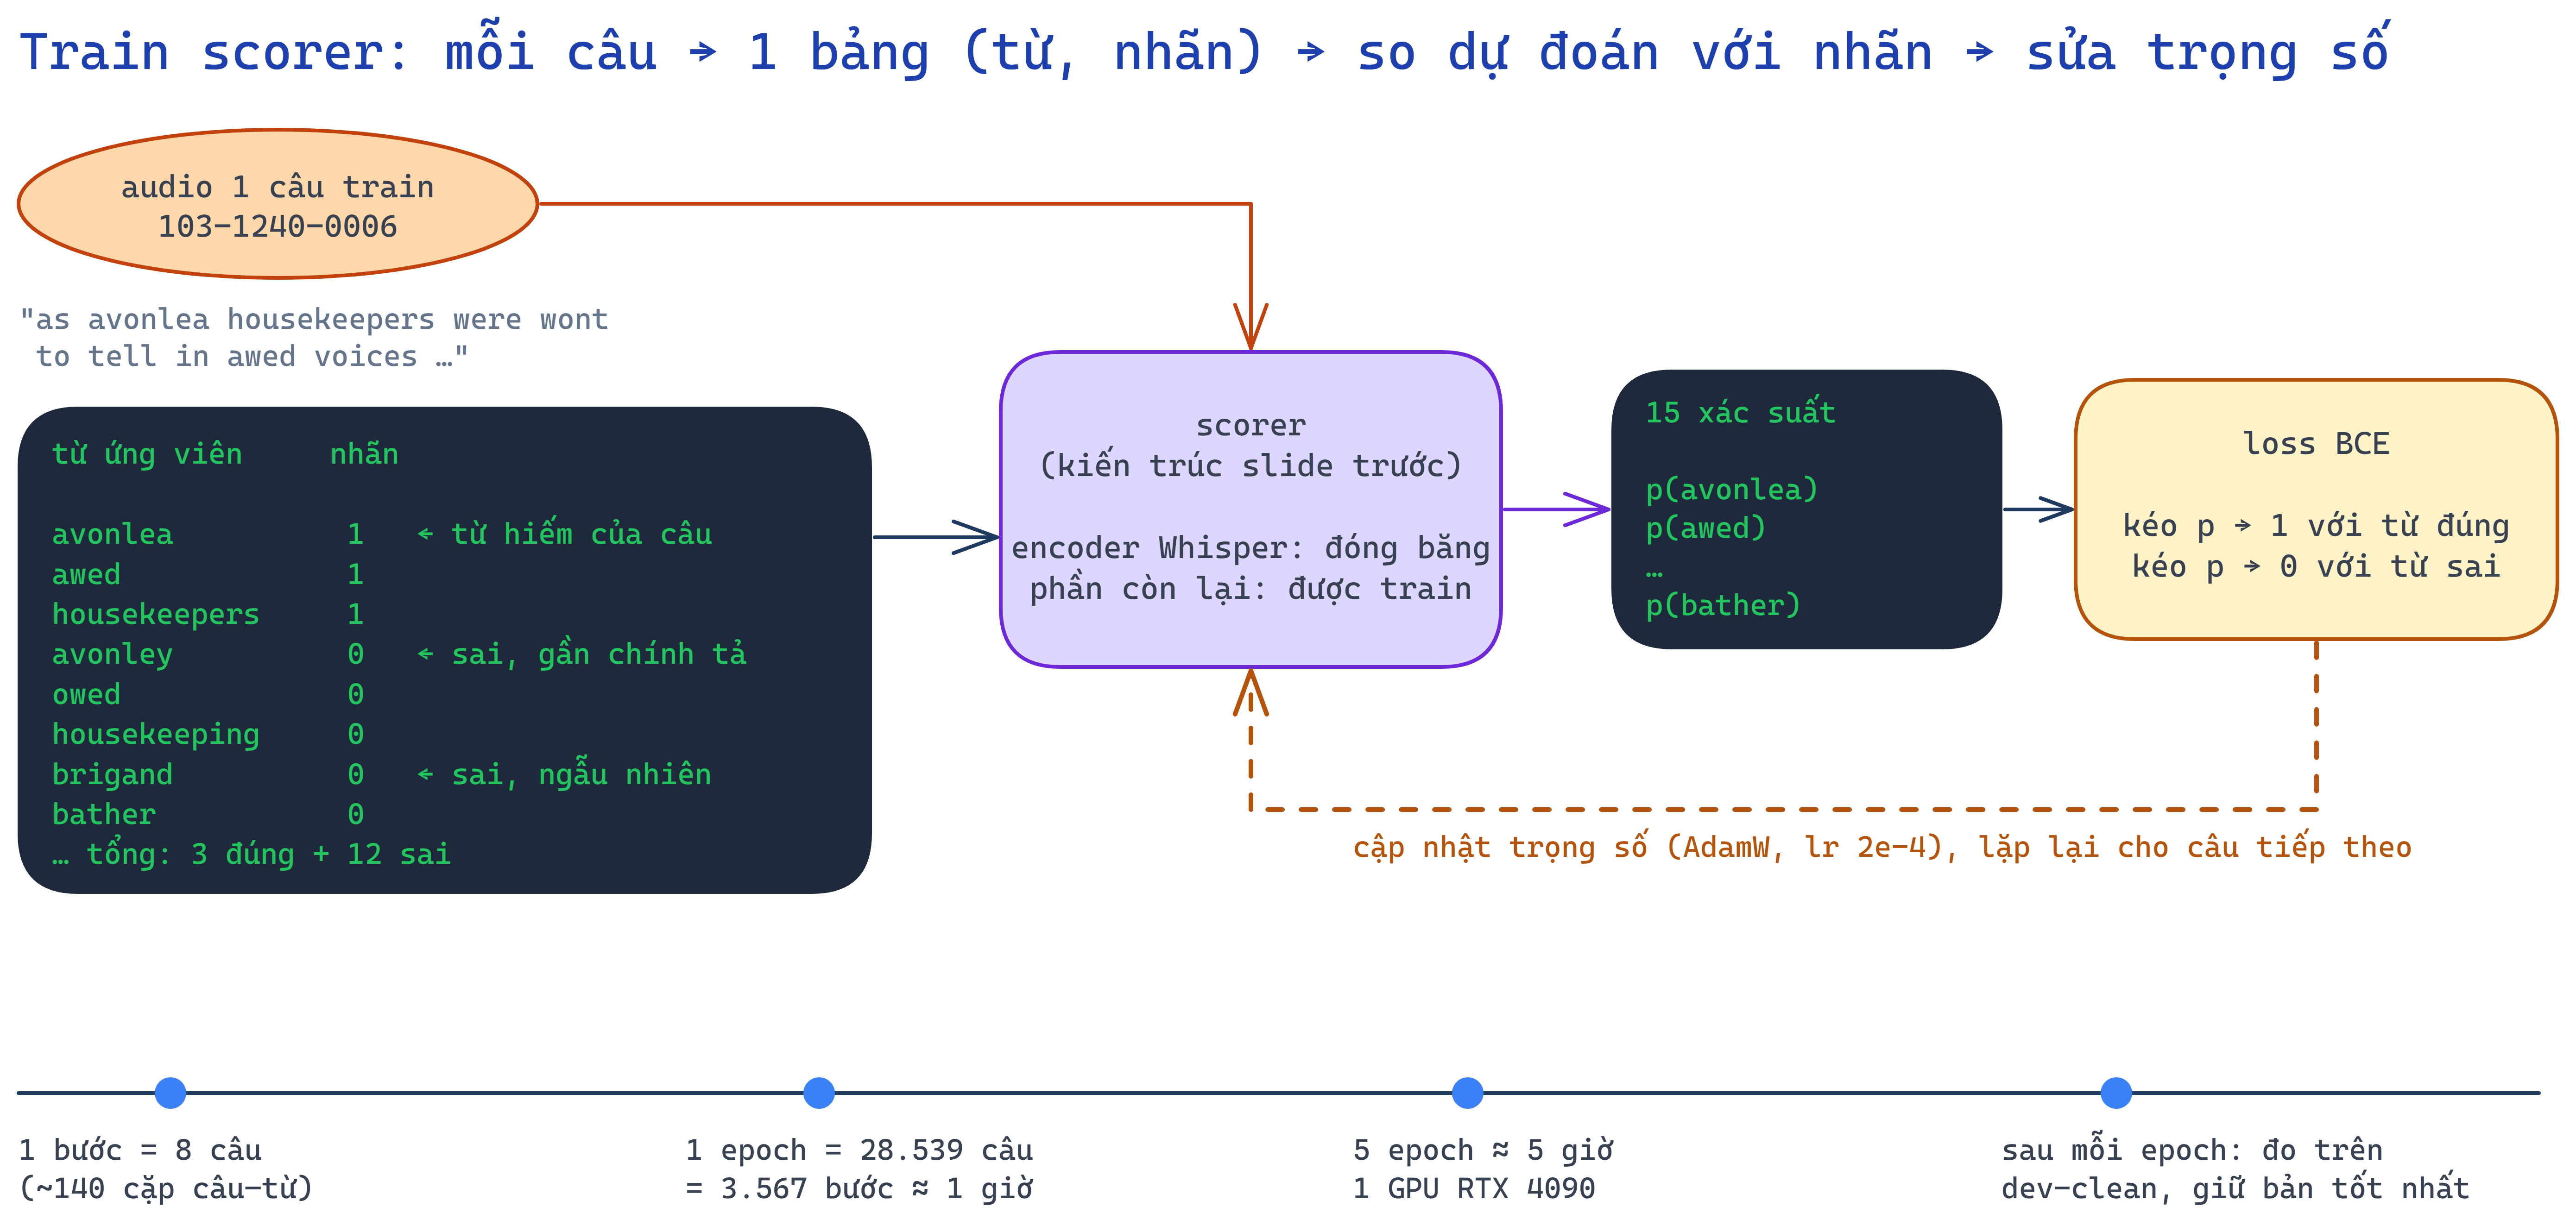
\includegraphics[height=0.70\textheight]{imgs/training.png}\\[2pt]
{\footnotesize Từ sai lấy giống Hou25 (40\% gần chính tả để model học phân biệt từ nghe gần giống). Mỗi câu: tối đa 8 từ đúng, số từ sai = 4 $\times$ số từ đúng.}
\end{frame}

\begin{frame}{Dùng thế nào khi chạy thật}
\centering
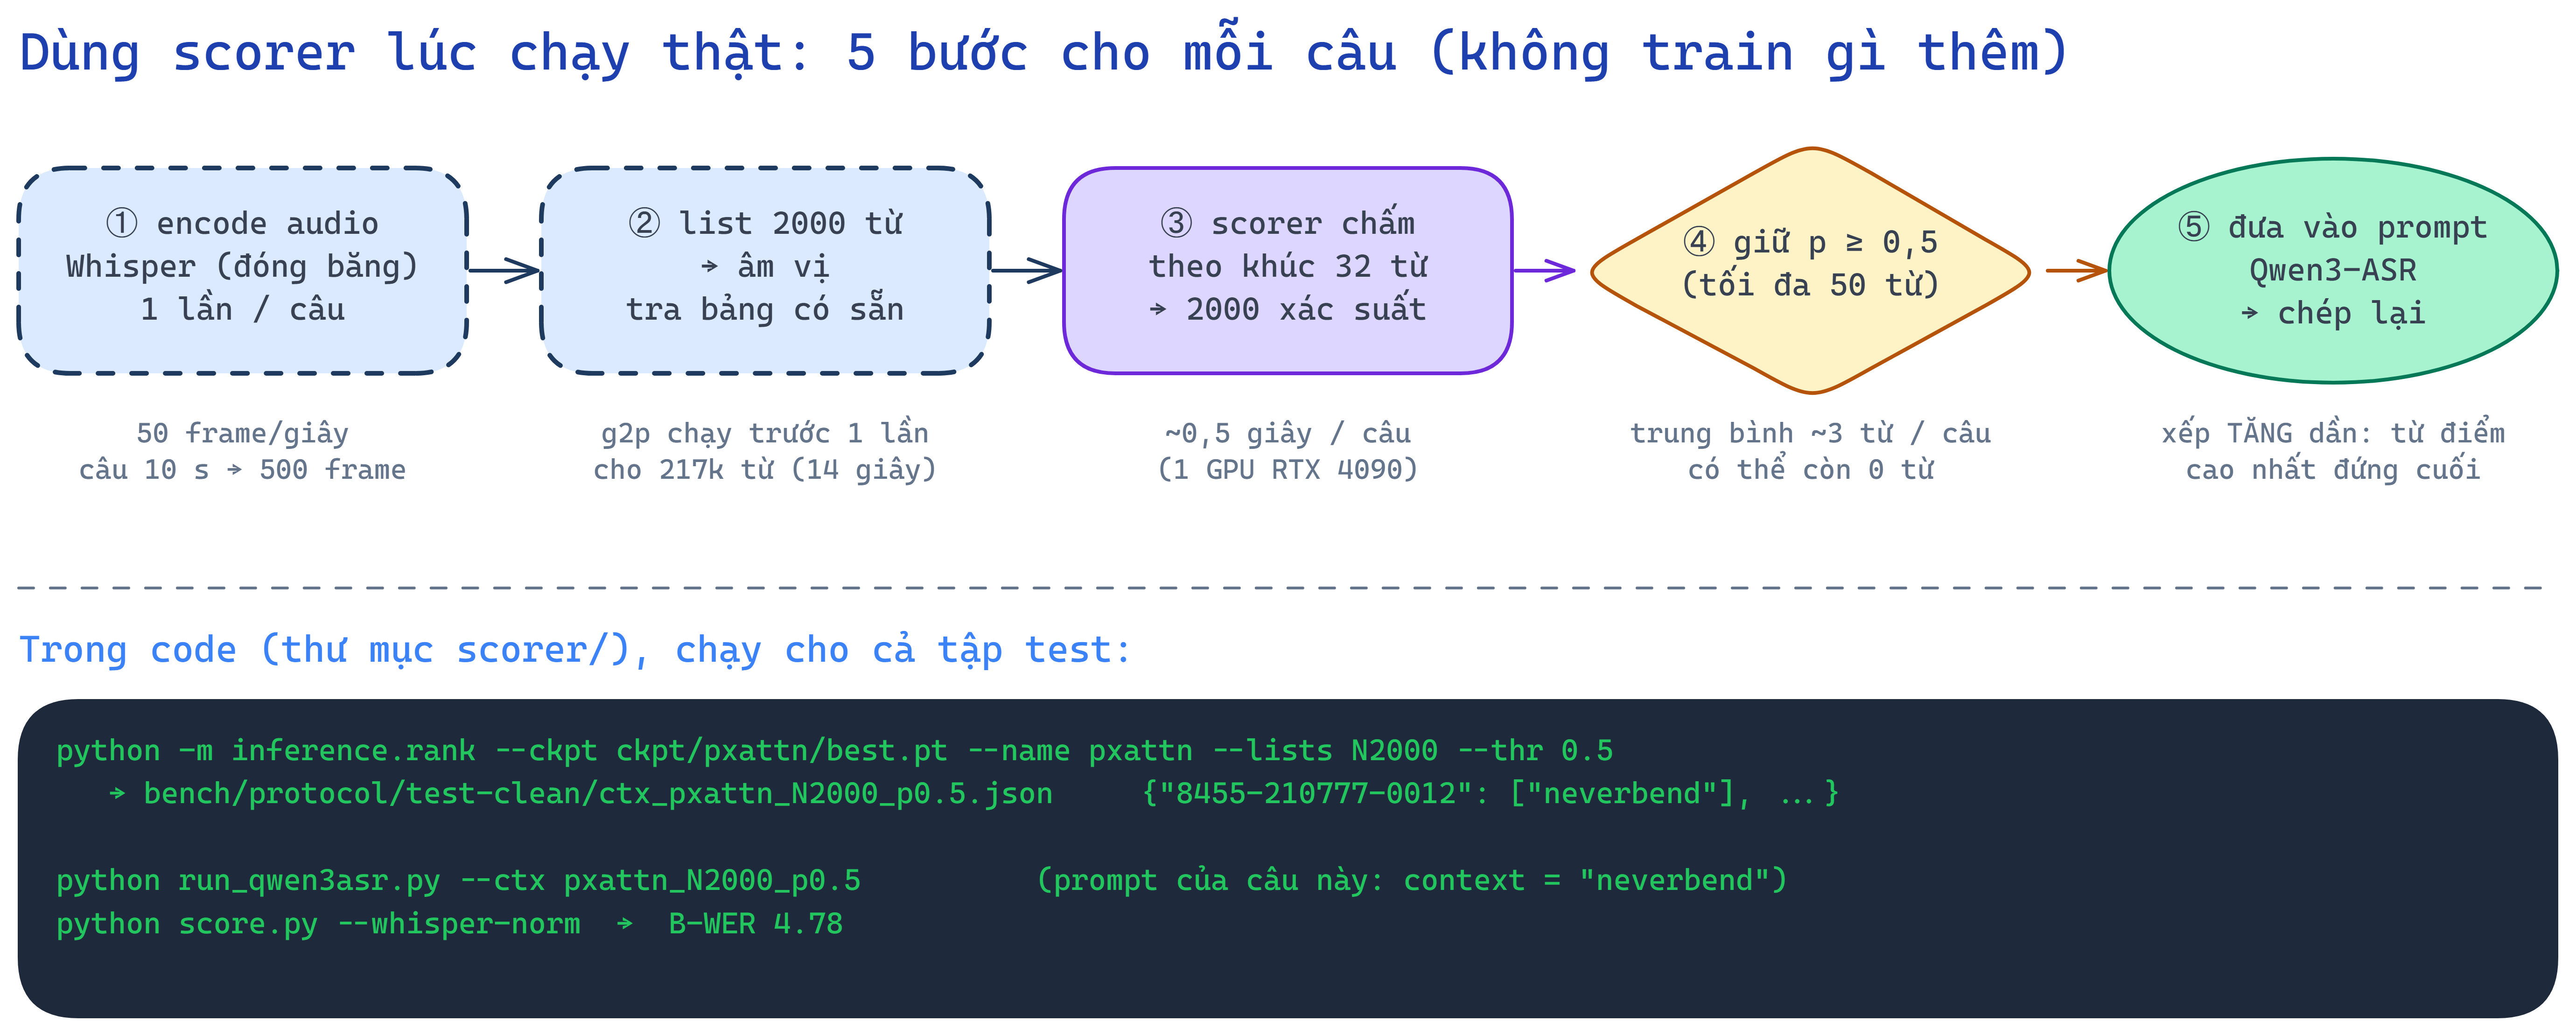
\includegraphics[width=\textwidth]{imgs/inference.png}
\end{frame}

\section{Kết quả}
\begin{frame}{Scorer chọn từ có đúng không? (test-clean, lọc p $\ge$ 0,5)}
\centering
\small\renewcommand{\arraystretch}{1.3}
\begin{tabular}{@{}lcccc@{}}
\toprule
\textbf{List đưa vào} & \textbf{Giữ / câu} & \textbf{Precision} & \textbf{Recall} & \textbf{Câu rỗng}\\
\midrule
100 từ & 2,1 & 98\% & 95\% & 25\%\\
2000 từ & 3,0 & 67\% & 95\% & 15\%\\
2000 từ, \textbf{không có từ đúng} & 1,0 & --- & --- & 46\%\\
\bottomrule
\end{tabular}
\vspace{0.4cm}
\begin{itemize}\itemsep4pt
\item \textbf{Precision}: từ giữ lại có đúng không. \textbf{Recall}: từ đúng có bị lọc mất không.
\item Từ 2000 từ còn $\sim$3 từ mà vẫn giữ \good{95\%} từ đúng.
\item Biết trả về \textbf{rỗng} khi list không có từ đúng (câu không có từ hiếm: 24\%).
\item List càng dài, từ giữ lại càng lẫn nhiễu: \bad{98\% $\rightarrow$ 67\%}.
\item Tốc độ: $\sim$0,5 giây/câu cho 2000 từ trên 1 GPU RTX 4090.
\end{itemize}
\src{test-other cùng xu hướng, thấp hơn: 2000 từ $\rightarrow$ 48\% / 89\%}
\end{frame}

\begin{frame}{Đưa list đã lọc vào Qwen3-ASR}
\centering
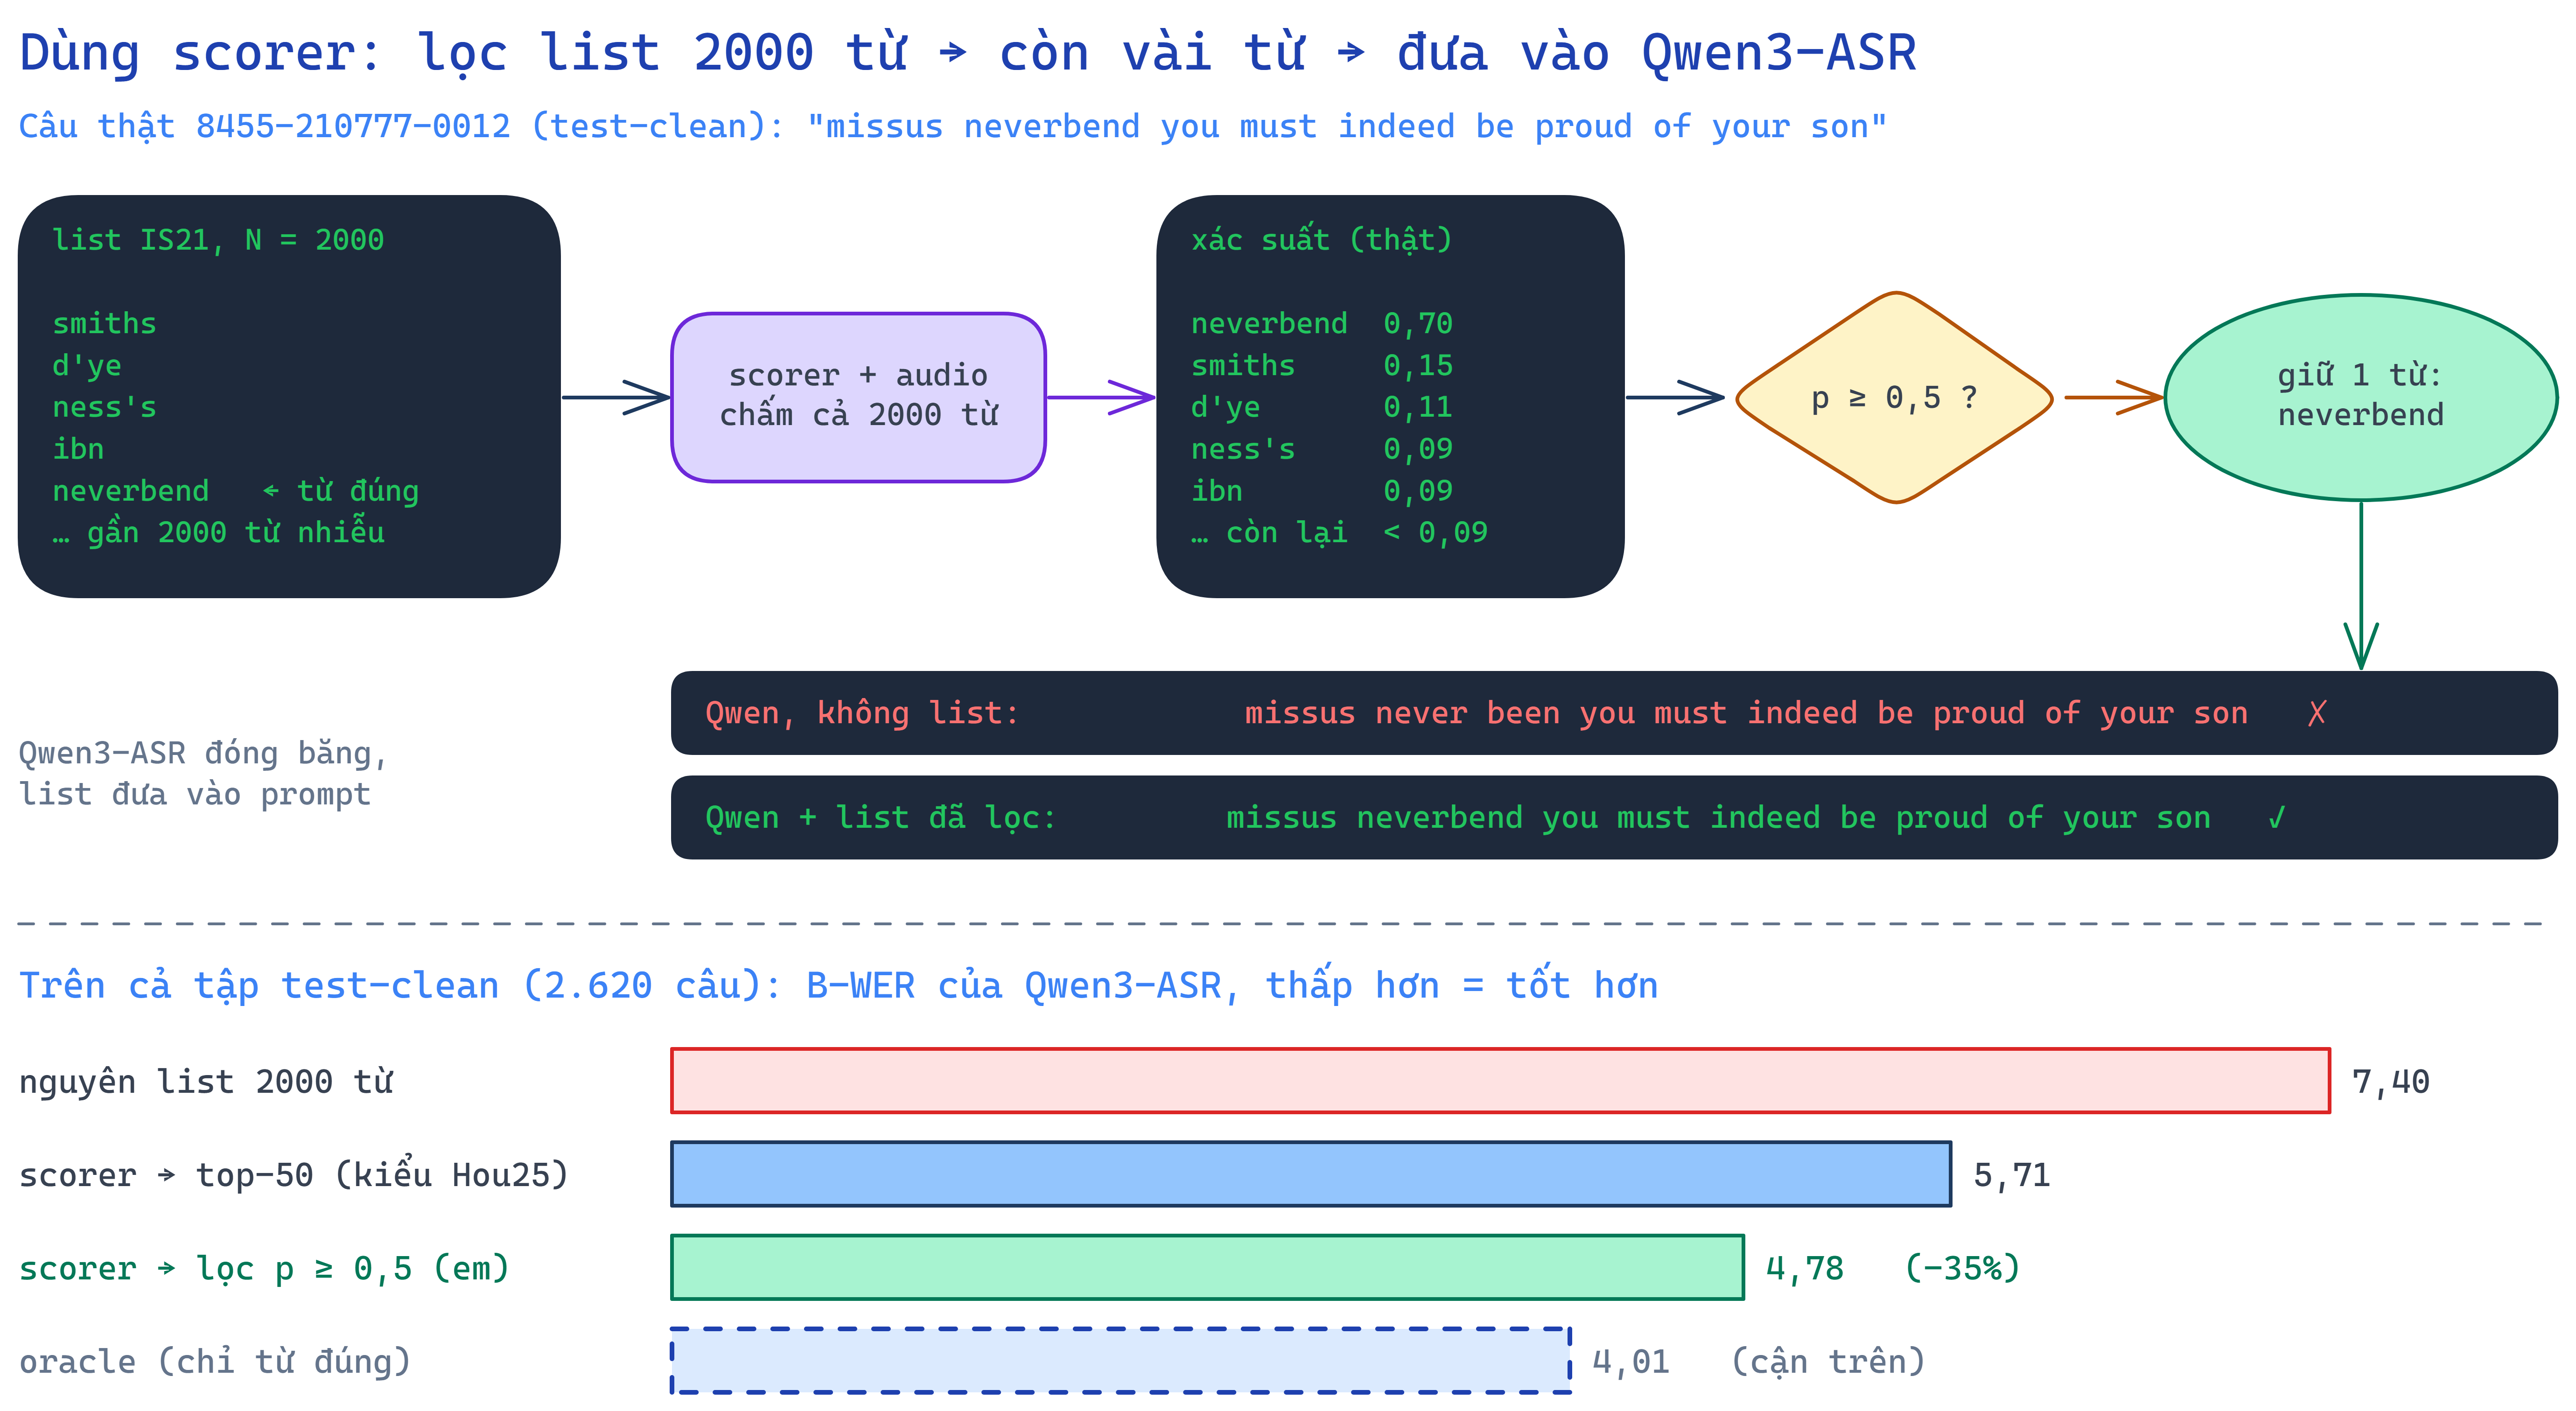
\includegraphics[height=0.76\textheight]{imgs/filter_pipeline.png}\\
{\footnotesize test-other: 16,45 $\rightarrow$ 11,57 (top-50) $\rightarrow$ \good{9,71} (lọc ngưỡng); oracle 7,73. (scorer IS21, wnorm)}
\end{frame}

\section{Tiếp theo}
\begin{frame}{Hạn chế và hướng tiếp theo}
\begin{columns}[T]
\begin{column}{0.5\textwidth}
\textbf{Hạn chế}
\begin{itemize}\itemsep4pt
\item List dài $\rightarrow$ độ chính xác tụt (98\% $\rightarrow$ 67\%).
\item Còn thua \textbf{PTC-Bias}: 4,10 / 7,76 (không cần train).
\item Đang thử cho scorer \textbf{xem thêm bản chép lần 1} của Qwen để ưu tiên từ Qwen chép sai $\rightarrow$ model \bad{học tắt} (dựa vào bản chép, bỏ qua audio): 6,58. Đang sửa.
\end{itemize}
\end{column}
\begin{column}{0.48\textwidth}
\textbf{Câu hỏi mở}
\begin{enumerate}\itemsep4pt
\item Lọc theo ngưỡng đã đủ làm đóng góp chính, hay cần vượt PTC-Bias trước?
\item Ưu tiên \textbf{cải thiện scorer}, hay \textbf{tự sinh list bằng LLM} khi không có list sẵn?
\item Có cần thêm Whisper để so trực tiếp với số của Hou25?
\end{enumerate}
\end{column}
\end{columns}
\end{frame}
\end{document}
